\documentclass[11pt,a4paper]{article}

% Encoding and fonts
\usepackage[utf8]{inputenc}
\usepackage[T1]{fontenc}
\usepackage{inconsolata}

% Math & formatting
\usepackage{amsmath, amssymb}
\usepackage{graphicx}
\usepackage{geometry}
\geometry{margin=1in}
\usepackage{url}
\usepackage{booktabs}

% Bibliography
\usepackage[
  backend=biber,
  style=numeric,
  sorting=none,
  doi=true,
  url=true
]{biblatex}
\addbibresource{references.bib}

% Hyperlinks (load last, once)
\usepackage[hidelinks]{hyperref}

% Title/author: use \texorpdfstring to make the PDF bookmark safe
\title{Supporting Information of AIedes: a neural-network framework for modelling the distribution and abundance of \textit{Aedes albopictus} in Europe}

\author{%
Indaco Biazzo\textsuperscript{1} \and
Lia Orfei\textsuperscript{1} \and
Ioannis Kioutsioukis\textsuperscript{2} \and
Lea Schuh\textsuperscript{1} \and
Céline Gossner\textsuperscript{3} \and
Olivier Briet\textsuperscript{3} \and
Peter V. Markov\textsuperscript{1,4}
}

\date{} % empty date to suppress today's date

\begin{document}

\maketitle

{\fontsize{7pt}{8pt}\selectfont\linespread{0.8}\noindent
\textsuperscript{1}European Commission, Joint Research Centre (JRC), Ispra, Italy; 
\textsuperscript{2}Department of Physics, University of Patras, Rio, Greece; 
\textsuperscript{3}European Centre for Disease Prevention and Control, Solna, Sweden; 
\textsuperscript{4}London School of Hygiene and Tropical Medicine, London, UK.
}

\section{Climate-Based Filtering of Distribution Data}

As introduced in the Data and Methods section, under the subsection \textit{Aedes albopictus datasets} and the paragraph \textit{Mosquito presence prediction}, the ECDC/EFSA VectorNet maps \cite{ecdc2024b, Wint2023} provide the baseline presence and absence information for \emph{Aedes albopictus} at the NUTS3 administrative level (NUTS2 for a few countries). To integrate these data with the Copernicus climate variables used in our model (spatial resolution of $12.5\,\text{km} \times 12.5\,\text{km}$), we reprojected the administrative-unit classifications onto the same regular grid as the Copernicus climate dataset, covering the European domain \cite{biazzo2026_datasets}.

Such spatial downscaling may introduce artefacts, particularly spurious presences in climatically unsuitable areas, due to the coarse administrative boundaries relative to environmental gradients. To mitigate these effects, following an approach similar to \cite{zardini2024}, we applied a climate suitability mask to filter out implausible conditions.

Specifically, any grid cell classified as ``present'' after downscaling was reassigned to ``absent'' if local climate conditions fell outside ecological thresholds established in \cite{ecdc2024a}. The mask combined two independent suitability functions:
\begin{itemize}
    \item precipitation suitability, requiring annual precipitation greater than or equal to $200~\text{mm}\,\text{yr}^{-1}$;
    \item temperature suitability, requiring both a mean temperature of the coldest month greater than or equal to $-3^{\circ}\text{C}$ to ensure egg overwintering, and an annual mean temperature greater than or equal to $10^{\circ}\text{C}$ to support development.
\end{itemize}

A grid cell was retained as suitable only if both precipitation and temperature criteria were met. This filtering step ensured internal consistency between the observed distribution and the climatic envelope of \emph{Ae. albopictus}, thereby reducing the impact of administrative-level downscaling artefacts before model training.

\section{Robustness of the \textit{\textbf{AI}edes}-Classifier to spatial autocorrelation}
\label{sec:si_spatial}

\subsection{Motivation and NUTS3-level data splitting}

Climate variables derived from gridded products such as Copernicus exhibit spatial autocorrelation, which can artificially inflate predictive performance when training and test samples are randomly drawn at the grid-cell level. To assess the robustness of the \textit{\textbf{AI}edes}-Classifier to this effect, we performed an additional sensitivity analysis in which training and test data were separated at the level of NUTS3 regions.

In this alternative setup, all grid cells belonging to a given NUTS3 region were assigned either to the training set or to the test set, ensuring that no administrative unit contributed data to both subsets. This represents a substantially more stringent validation scenario, as the model must generalize across entire regions rather than across nearby grid cells that share similar climatic conditions and aggregated labels. All analyses were repeated using five different random assignments of NUTS3 regions to training and test sets.

\subsection{Training dynamics and model selection under NUTS3 splitting}

Figure~\ref{fig:si_loss_training} shows the training dynamics and model selection results obtained under the NUTS3-level split. Panel~(a) reports representative training and testing loss curves for a neural network trained on temperature and total precipitation inputs. As in the main analysis, the loss decreases smoothly and stabilizes after the initial epochs, with the testing loss remaining slightly higher than the training loss, indicating the absence of overfitting despite the stricter spatial separation.

Panel~(b) reports test accuracy as a function of the total number of model parameters (log scale), for different neural network architectures and input configurations. As observed in the main text, increasing the number of hidden layers and units improves predictive performance, and including precipitation as an additional input variable consistently enhances accuracy. Under the NUTS3 split, the best-performing architectures consistently feature three hidden layers, with the highest scores obtained for configurations with 40 units per layer ([40,\,40,\,40]). When accounting for variability across folds, performance differences between this architecture and the [50,\,50,\,50] configuration identified under random splitting fall within the corresponding standard deviations, indicating that the two models are statistically compatible and achieve comparable predictive performance.

\begin{figure}[h]
    \centering
    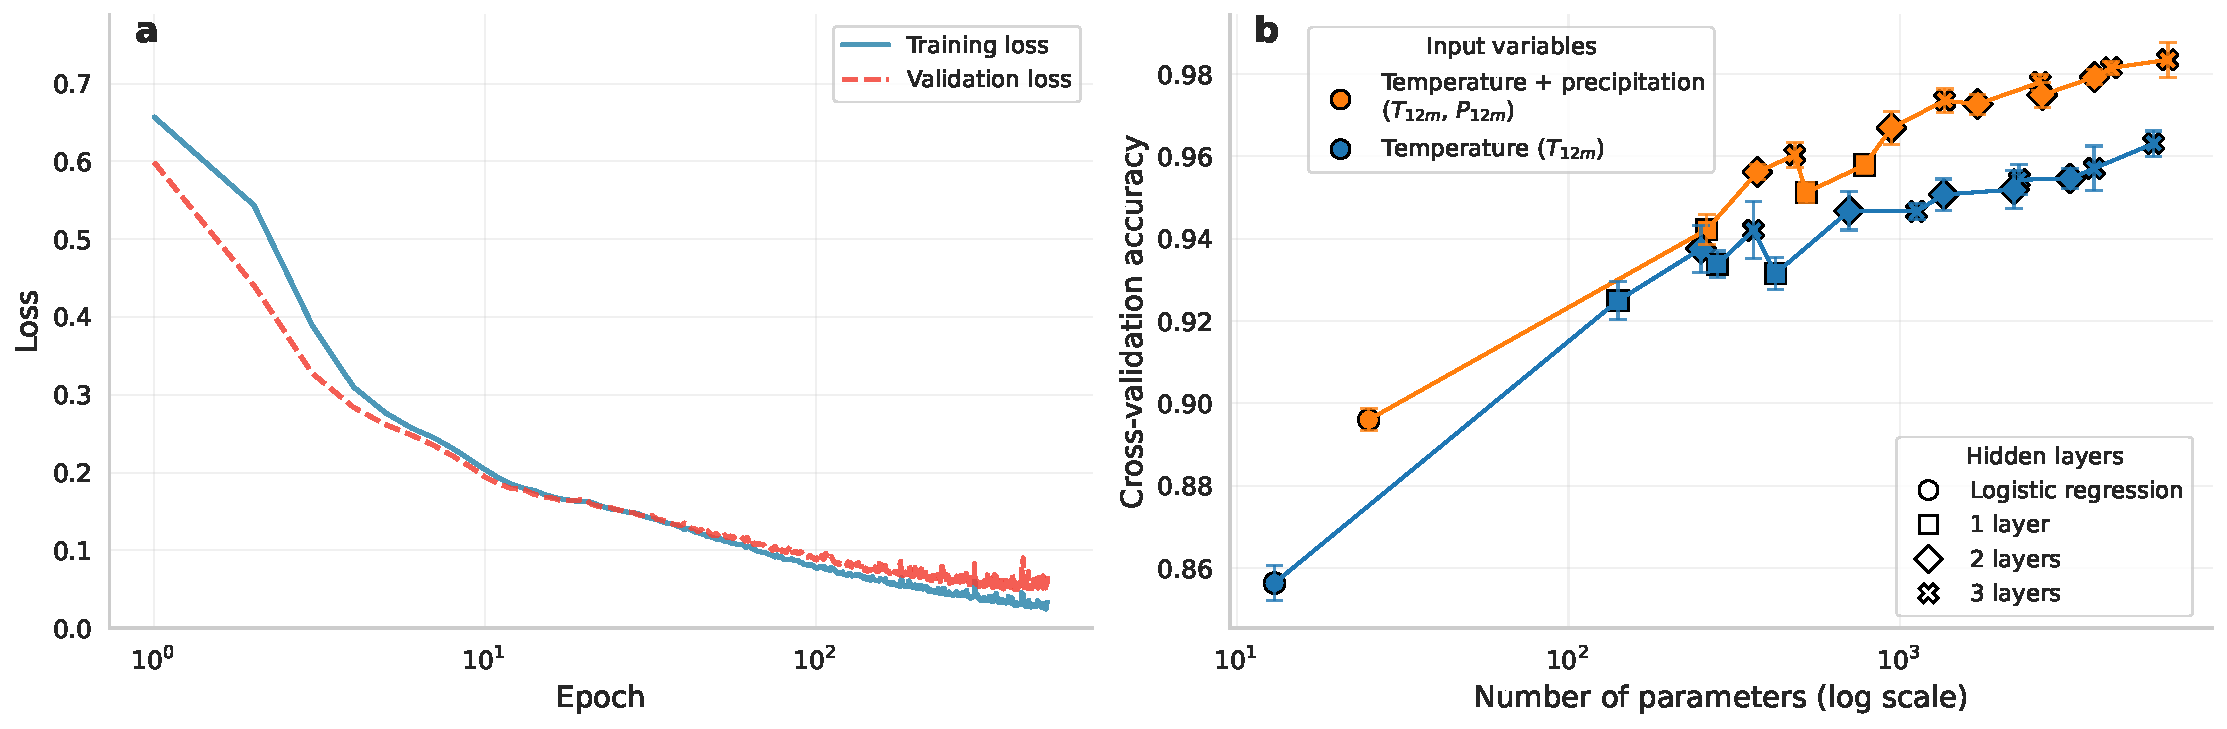
\includegraphics[width=\linewidth]{img/combined_loss_acc_nuts3.pdf}
    \caption{
    \textbf{Training dynamics and model performance of the \textit{\textbf{AI}edes}-Classifier under NUTS3-level splitting.}
    \textbf{(a)} Example of training and testing loss curves over the training epochs for a neural network model trained on temperature and total precipitation inputs. The dataset is split into training and test sets at the NUTS3 level. The stabilization of the testing loss indicates the absence of overfitting.
    \textbf{(b)} Test accuracy as a function of the total number of model parameters (log scale), for different neural network architectures and input-variable configurations. Each point corresponds to a distinct architecture with varying numbers of hidden layers and units. Including precipitation and increasing model complexity improves predictive performance.}
    \label{fig:si_loss_training}
\end{figure}

\subsection{Performance comparison across splitting strategies}

Model performance was evaluated using accuracy, specificity, sensitivity, and critical success index (CSI). Metrics were computed over the entire dataset (aggregating predictions across all folds) and on the held-out test sets only.

When computed over the full dataset (five-fold average), the following values were obtained:

\begin{itemize}
    \item \textbf{Random 80/20 split:} accuracy 0.993, specificity 0.996, sensitivity 0.989, CSI 0.981.
    \item \textbf{NUTS3-level split:} accuracy 0.973, specificity 0.983, sensitivity 0.954, CSI 0.926.
\end{itemize}

As expected, enforcing spatial separation at the NUTS3 level leads to a reduction in all performance metrics. Nevertheless, values remain high across all indicators, confirming that the classifier retains strong predictive ability even under strict spatial constraints. We consider whole-dataset metrics to be the most reliable summary of model performance in this context, as misclassifications under the NUTS3 split are concentrated in a limited number of regions, whose assignment to the training or test set can disproportionately affect test-only metrics.

For completeness, we also report the best test-set-only results obtained under each splitting strategy:

\begin{itemize}
    \item \textbf{NUTS3 split} (best architecture [40,\,40,\,40]): accuracy 99.20\%, specificity 0.987, sensitivity 0.994, CSI 0.982.
    \item \textbf{Random split} (best architecture [50,\,50,\,50]): accuracy 98.81\%, specificity 0.983, sensitivity 0.991, CSI 0.974.
\end{itemize}

While these test-set results confirm strong predictive performance under both strategies, their dependence on the specific regions held out reinforces the use of whole-dataset averages as the primary indicator of robustness.

\subsection{Spatial predictions under NUTS3-level splitting}

Figure~\ref{fig:si_nn_accuracy_map} reproduces the spatial comparison shown in the main text, but using predictions from models trained under the NUTS3-level split. Panel~(a) shows predictions from the simplest neural network architecture, equivalent to logistic regression, while panel~(b) shows predictions from the best-performing deep neural network, featuring three hidden layers with 40 units each. Panel~(c) summarizes the corresponding performance metrics, which in this case are computed over the entire dataset by aggregating predictions across all folds. This differs from the main-text figure, where metrics are reported on the held-out test set, and reflects our choice to use whole-dataset averages here in order to obtain more stable estimates under NUTS3-level splitting, given the limited number of regions driving most misclassifications.


The spatial patterns of predicted presence probability are qualitatively consistent with those obtained under random splitting. Differences are confined to a limited number of marginal regions, typically characterized by low predicted suitability or by areas where the invasion process is likely incomplete.

\begin{figure}[h]
    \centering
    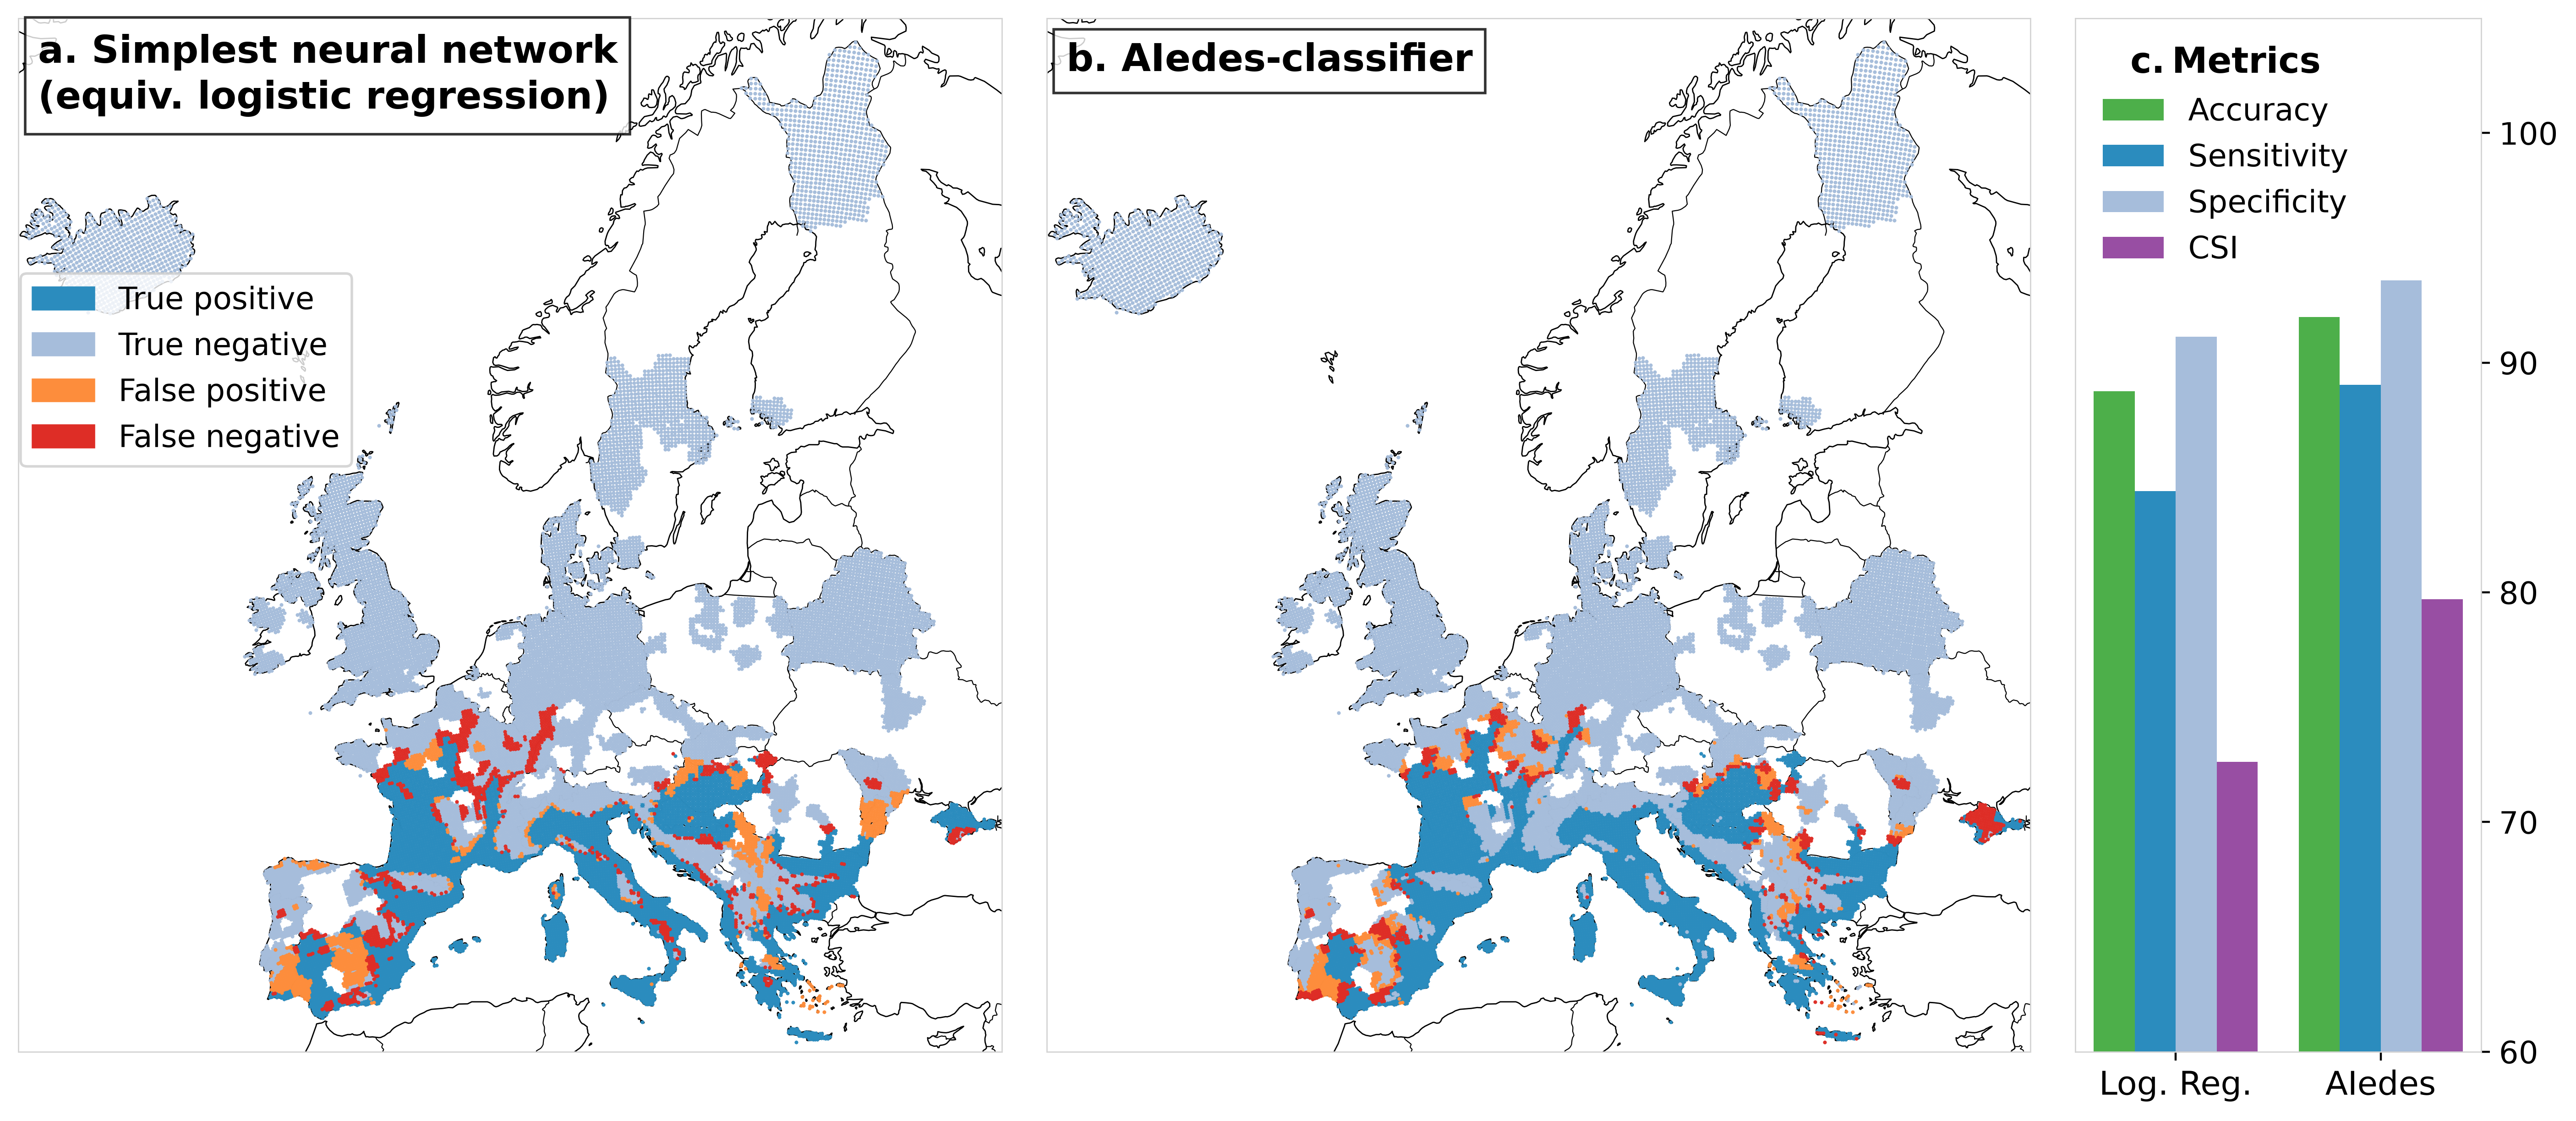
\includegraphics[width=0.95\textwidth]{img/comparison_lr_nn_nuts3.png}
    \caption{
    \textbf{Predicted probability of presence of \textit{Ae. albopictus} under NUTS3-level train--test separation.}
    \textbf{(a)} Predictions from the simplest neural network architecture tested, featuring no hidden layers and statistically equivalent to logistic regression.
    \textbf{(b)} Predictions from the best-performing \textit{\textbf{AI}edes}-Classifier model under spatial splitting, consisting of three hidden layers with 40 units each.
    \textbf{(c)} Performance metrics (accuracy, sensitivity, specificity and critical success index, CSI) computed against observed presence--absence data.}
    \label{fig:si_nn_accuracy_map}
\end{figure}

\subsection{Summary}

This sensitivity analysis demonstrates that the strong performance gains achieved by the \textit{\textbf{AI}edes}-Classifier over simpler models are not driven by spatial autocorrelation or information leakage between training and test data. While the random split used in the main text remains appropriate for evaluating in-domain interpolation under current surveillance conditions, the NUTS3-level split confirms that the model generalizes well across administrative regions and retains high predictive accuracy under stricter validation criteria.


\section{Comparison with WorldClim-Based Distribution Modelling}

In the main text, we compared the performance of the \texttt{AIedes}-classifier with that of a logistic regression model, i.e. the same functional form adopted by \cite{zardini2024}, but applied to different climatic input datasets.

The model by \cite{zardini2024} was developed using the \textit{WorldClim} bioclimatic dataset \cite{worldclim_2023}, which provides long-term averaged climatic conditions for the period 1970–2000. In contrast, our analyses rely on Copernicus-based climate variables, which better reflect the current environmental conditions corresponding to the mosquito records collected in 2023. Moreover, Copernicus products offer greater flexibility for future predictive applications, given their wide range of climate projection models and continuous availability for upcoming years.

In \cite{zardini2024}, four WorldClim variables were used as key climatic predictors: annual mean temperature, maximum temperature of the warmest month, annual precipitation, and precipitation of the warmest quarter (available at \url{https://www.worldclim.org/}). To ensure a consistent comparison, we repeated our analysis using these same WorldClim variables.

Figure~\ref{fig:map_comparison_SI} compares our predicted distribution of \emph{Aedes albopictus} presence with the distribution reported by \cite{zardini2024}. The resulting probability map indicates that the improvements achieved by our framework remain consistent when applied within the original WorldClim-based setting.

\begin{figure}[h!]
    \centering
    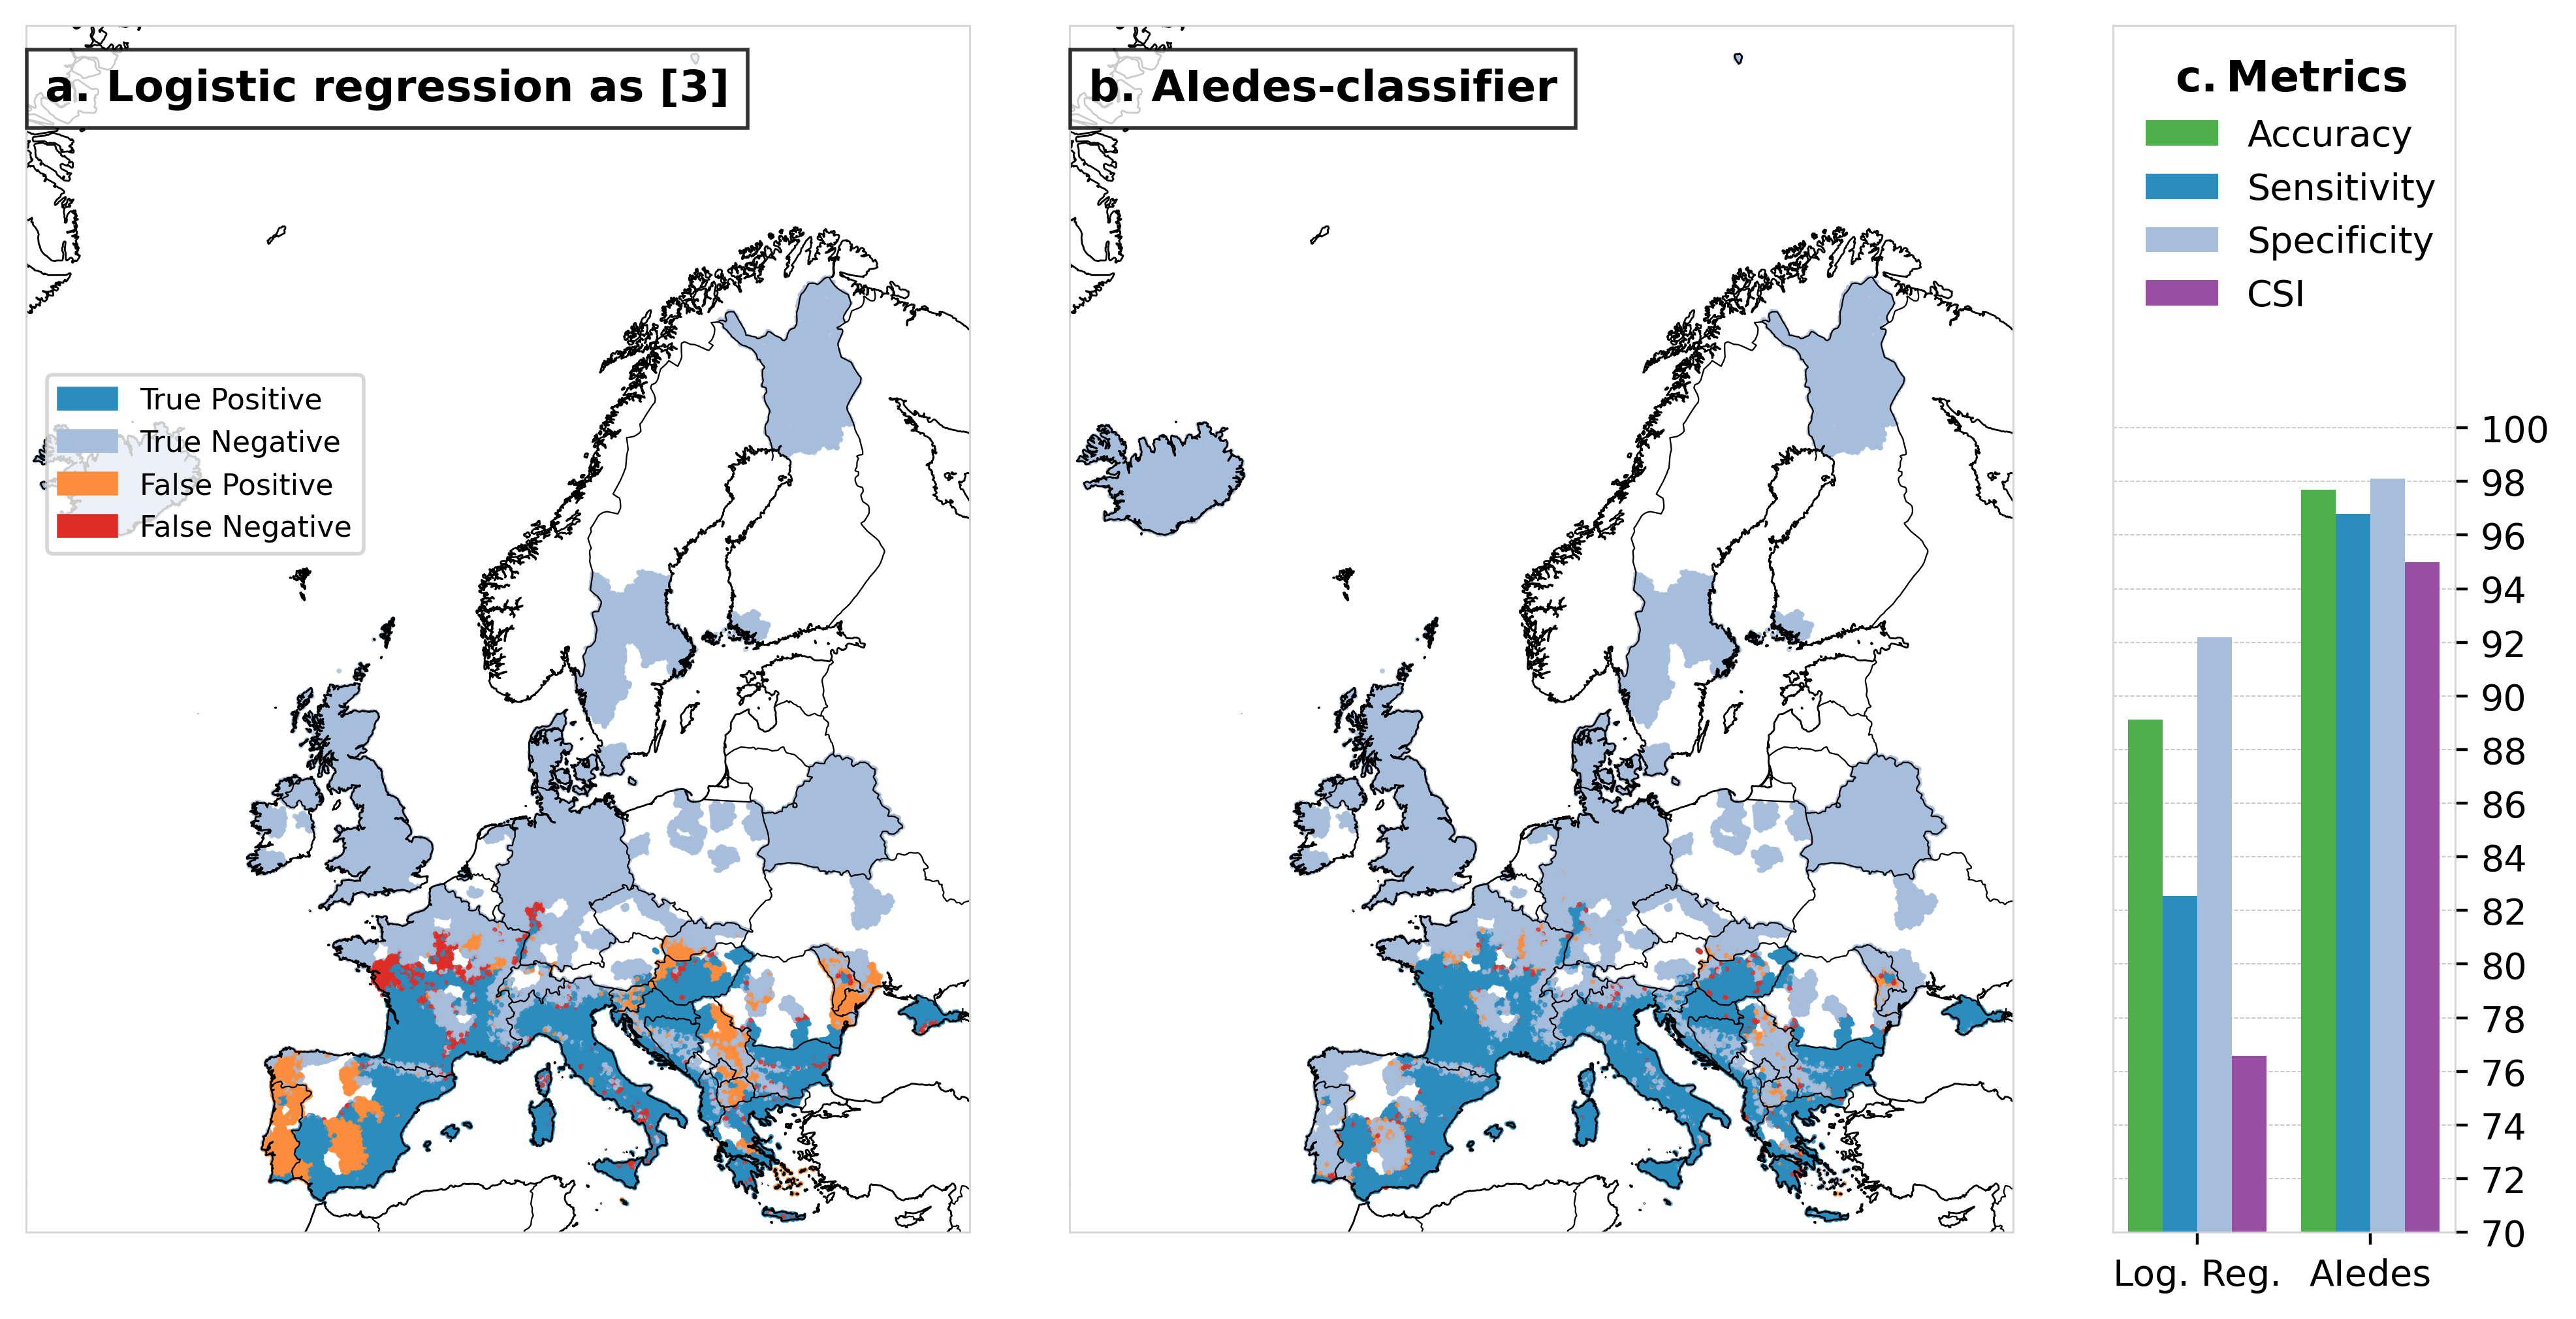
\includegraphics[width=0.85\linewidth]{img/comparison_lg_aiedes_worldClim.png}
    \caption{Comparison between the predicted presence maps produced by the \texttt{AIedes}-classifier (right) and the distribution reported by \cite{zardini2024} (left). The results confirm that the improvements identified in the main analysis are preserved when the original WorldClim-based climatic variables are employed.}
    \label{fig:map_comparison_SI}
\end{figure}



\section{Evaluation of Abundance Predictions}

In the Results section of the main text, we reported the performance of the \texttt{AIedes}-counter in predicting mosquito abundance, specifically the weekly laying-egg rates. In the corresponding scatter plots shown in the main text, the model appears to slightly underpredict the observed values, particularly at higher egg counts. To determine whether this apparent deviation reflects a systematic bias or falls within the expected range of natural variability, we performed a Bland–Altman analysis on the test set (Fig.~\ref{fig:bland_altman}).

The Bland–Altman plot compares the differences between predicted and observed egg counts against their mean values, thus enabling a direct evaluation of agreement beyond simple correlation metrics. The mean difference between predictions and observations was close to zero ($-0.79$), indicating the absence of systematic bias. The 95\% limits of agreement ($\pm1.96$ SD) ranged from approximately $-39$ to $+37$, capturing the natural variability inherent in oviposition data.  

Overall, the analysis confirms that the \texttt{AIedes}-counter provides unbiased abundance predictions across the full dynamic range of observations. The observed dispersion reflects stochastic fluctuations in egg counts rather than structural model errors, supporting the robustness of our abundance predictions even in the presence of occasional over- or underestimation at extreme values.

\begin{figure}[h!]
    \centering
    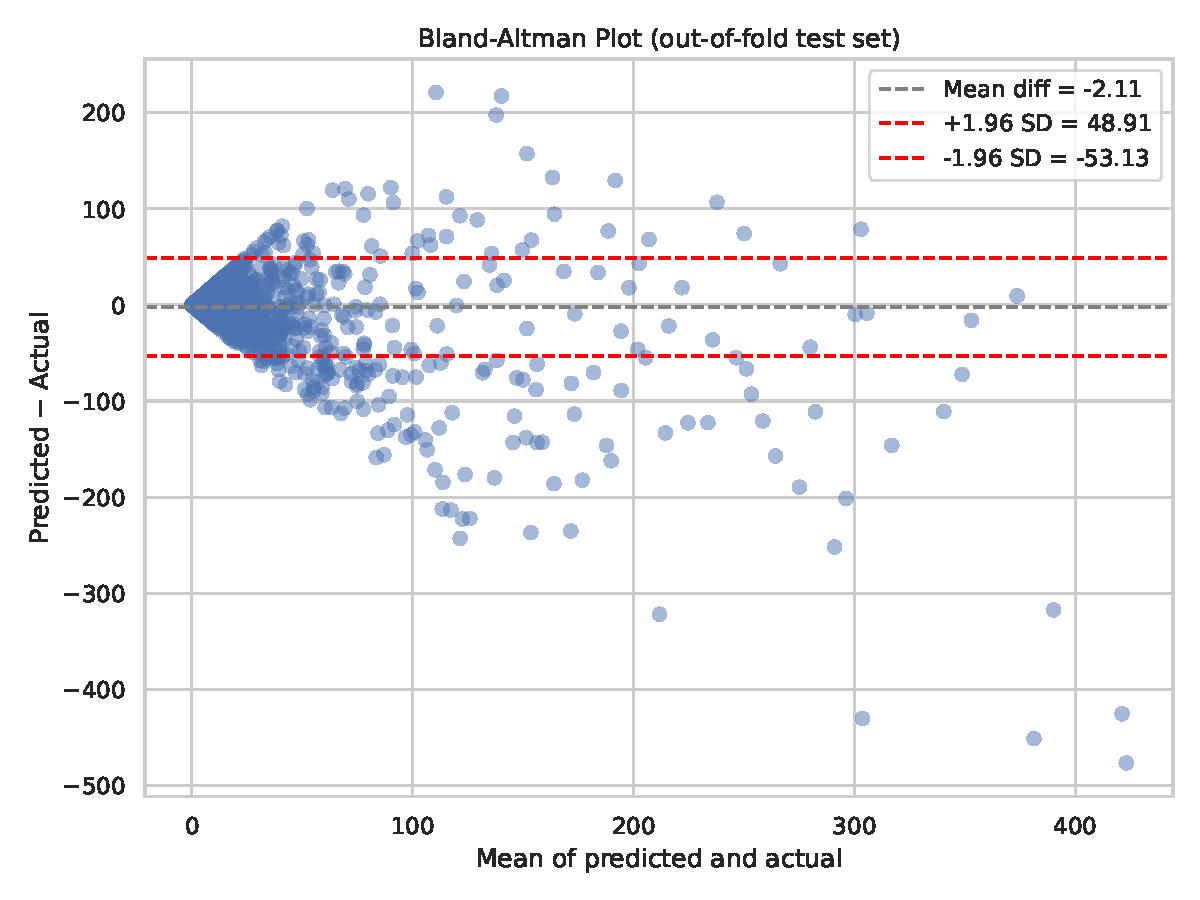
\includegraphics[width=0.65\linewidth]{img/bland_altman_test.pdf}
    \caption{Bland–Altman plot comparing predicted and observed egg counts in the test set. The mean difference ($-0.79$) indicates the absence of systematic bias, while the 95\% limits of agreement (dashed lines) reflect variability consistent with the stochasticity of oviposition data.}
    \label{fig:bland_altman}
\end{figure}

\section{Performance Across Loss Functions and Training Configurations for \texttt{AIedes}-counter}

We systematically evaluated the performance of the \texttt{AIedes}-counter under a range of training configurations. Each configuration was trained using multiple loss functions—\textit{Weighted Mean Squared Error} (WMSE), \textit{Weighted Mean Squared Logarithmic Error} (WMSLE), and \textit{Zero-Inflated Negative Binomial} (ZINB)—together with different dropout rates ($0.0$, $0.2$, $0.4$) and network depths (two or three hidden layers, each with 32 or 64 hidden units). For each combination, 20 independent models were trained with different random seeds to ensure the robustness of the results.

The input variables were tested in nine distinct combinations. The first configuration included only egg-laying rates from the previous one and two weeks. The second group comprised exclusively climatic predictors—mean near-surface air temperature, dew point temperature, and precipitation—while the third group combined both climatic and lagged egg-laying features. As detailed in the Data section, both daily and weekly averages of the climatic variables were considered.

Loss-specific learning rates were optimized for training stability and predictive performance: $1 \times 10^{-4}$ for WMSE, $1 \times 10^{-3}$ for WMSLE, and $5 \times 10^{-4}$ for ZINB.

Figures~\ref{fig:loss_dropout_r2} and \ref{fig:loss_dropout_acc} summarize the influence of these design choices on test $R^2$ and classification accuracy. Overall, dropout improved model generalization, with a rate of $0.2$ emerging as the most effective value. A similar pattern was observed across all configurations: using only the previous egg-laying rates resulted in substantially lower predictive performance compared to models trained with climatic predictors. Incorporating additional input variables progressively improved performance up to a certain extent, beyond which overfitting effects occasionally led to a slight decrease in predictive accuracy. The best results were consistently obtained when both climatic and lagged egg-laying variables were included, regardless of the loss function.

In general, both the \textit{Weighted Mean Squared Error} (WMSE) and the \textit{Weighted Mean Squared Logarithmic Error} (WMSLE) losses achieved higher $R^2$ values compared with the \textit{Zero-Inflated Negative Binomial} (ZINB) loss. When considering classification accuracy—i.e.\ the model’s ability to correctly predict zero versus non-zero egg counts—the WMSLE clearly outperformed the other loss functions. Based on these results, WMSLE was selected for the main analysis, as it provided the most accurate classification of presence/absence while maintaining strong agreement with observed abundance values. Importantly, the other loss functions yielded comparable results within their respective standard error ranges, further supporting the robustness of the modelling framework.

Table~\ref{tab:best_per_loss} lists the best-performing configuration for each loss function in terms of test $R^2$. As shown, WMSE and WMSLE achieved the highest $R^2$ values, with WMSE performing slightly better but not at a statistically significant level. In contrast, WMSLE exhibited a clear advantage in classification accuracy. These results guided our choice of WMSLE and the corresponding trained model for the analyses presented in the main text.

\begin{figure}
    \centering
    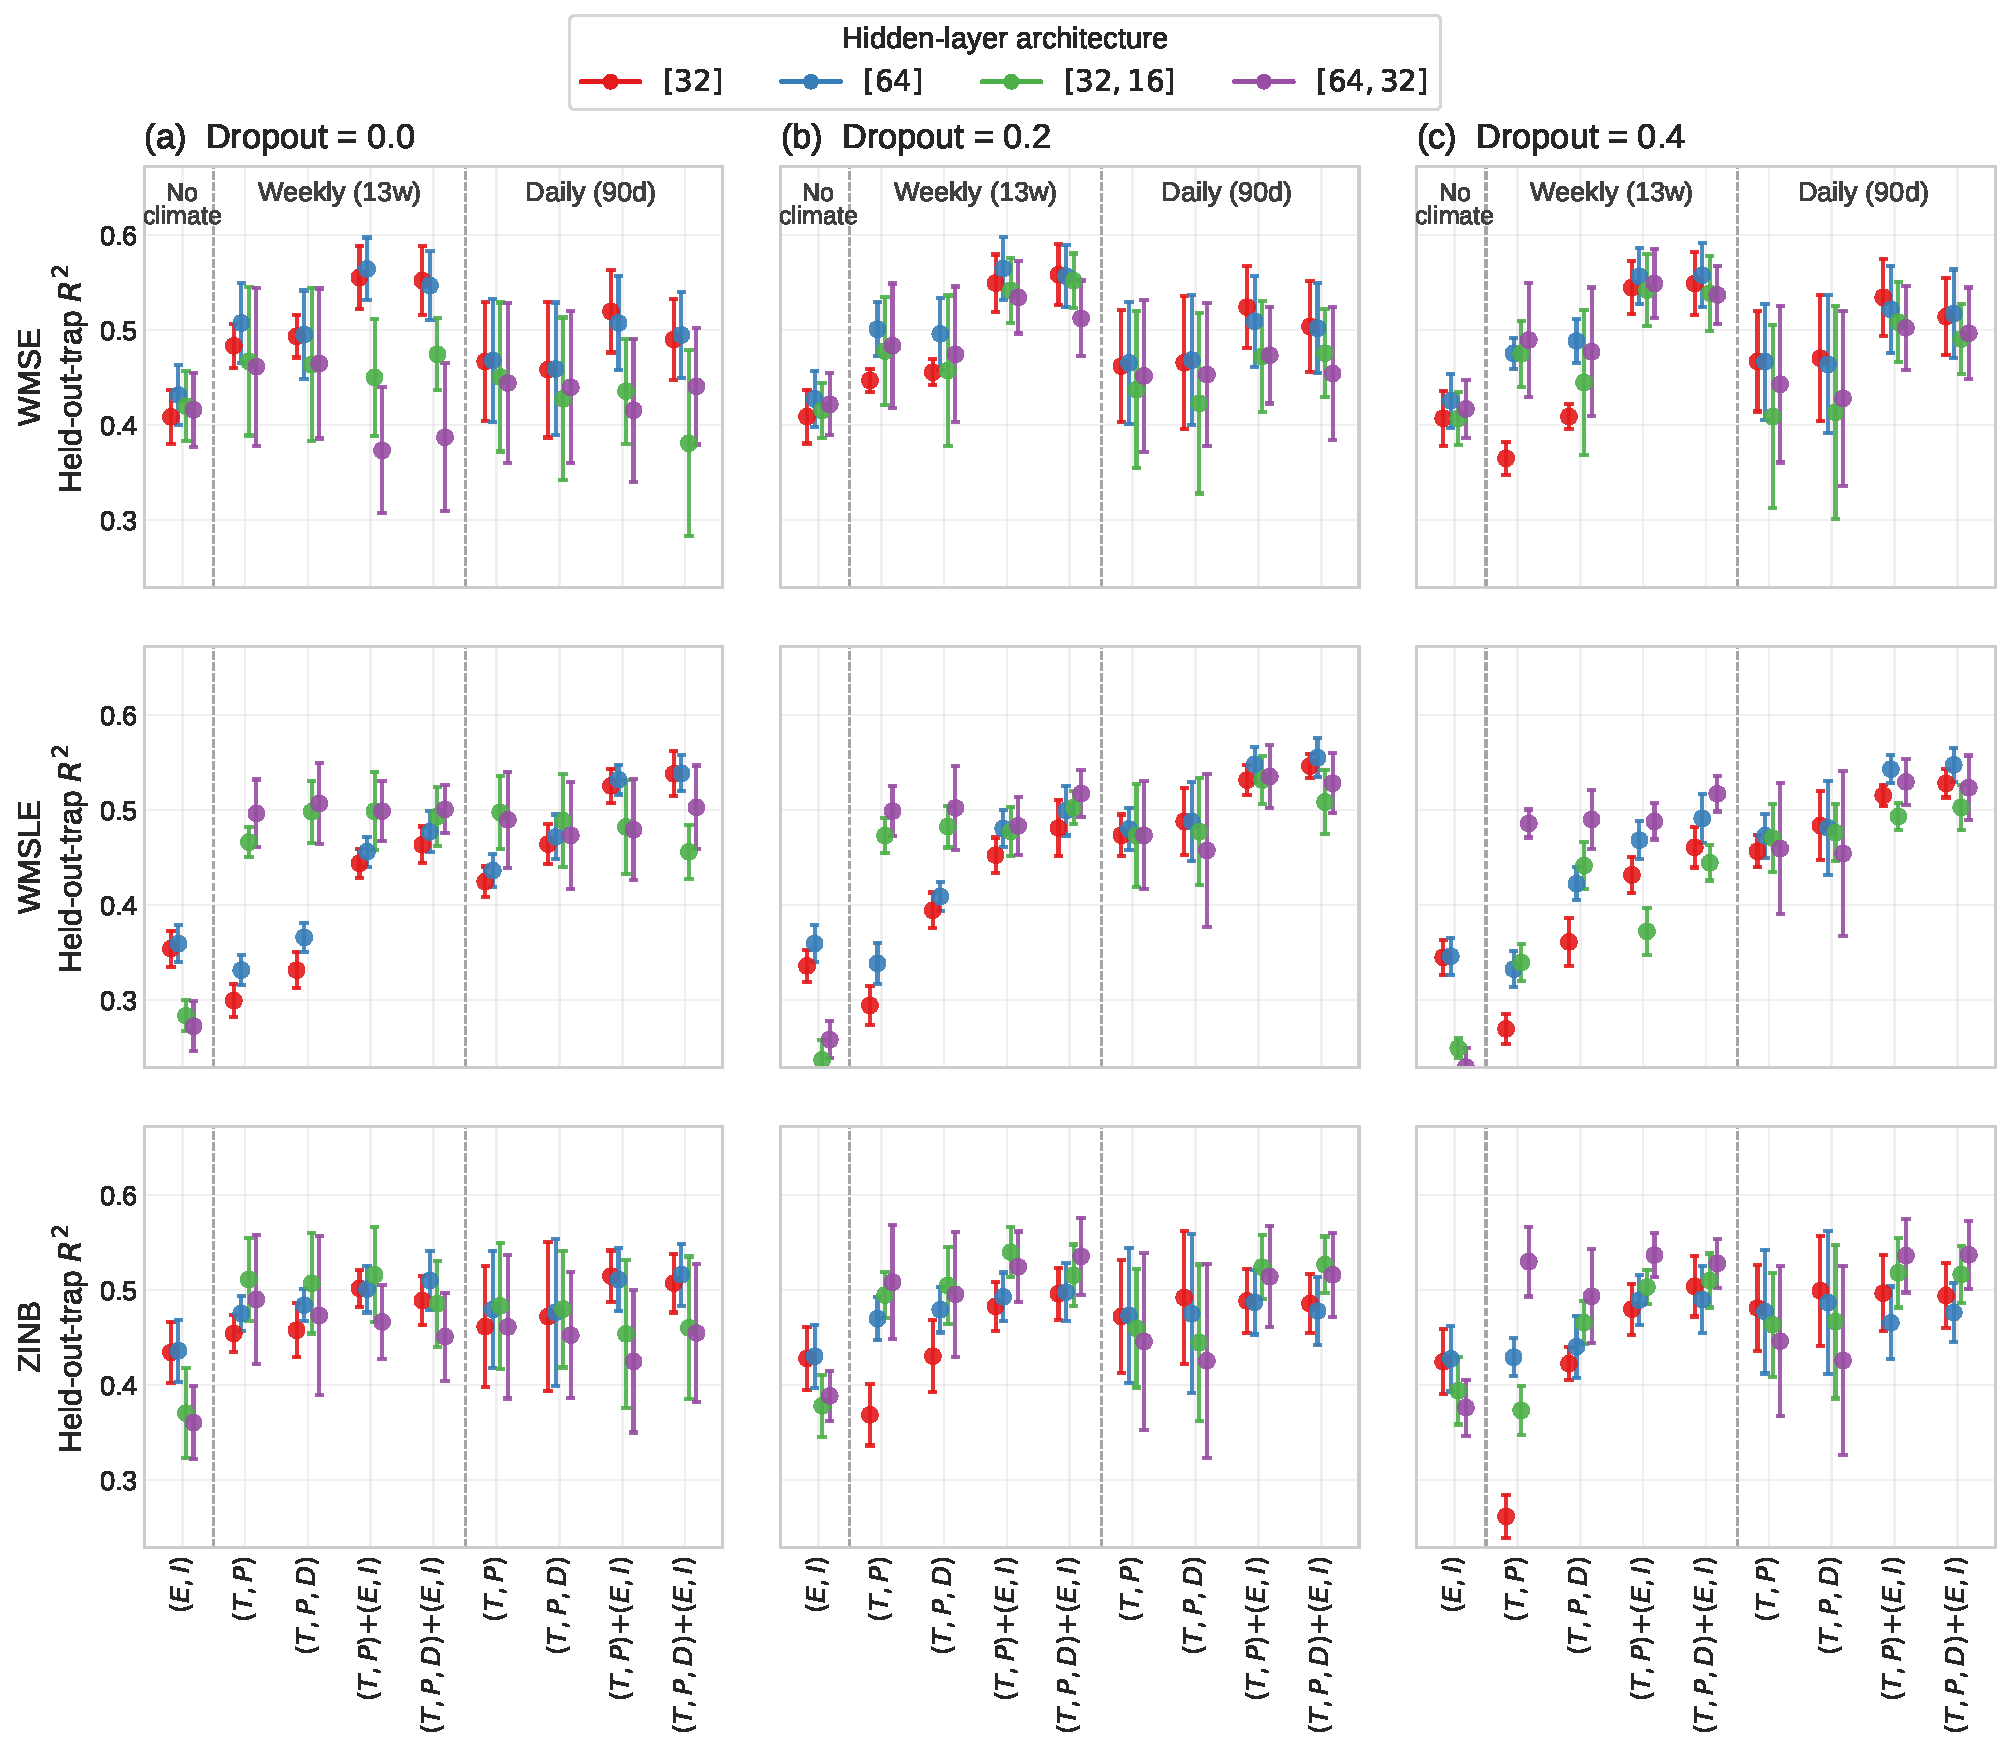
\includegraphics[width=0.8\linewidth]{img/nn_results_by_dropout_3loss.pdf}
    \caption{Effect of dropout, network depth, and input variable combinations on test $R^2$ across three loss functions (WMSE, WMSLE, ZINB). Moderate dropout ($0.2$) improved performance, while excessive dropout reduced predictive power.}
    \label{fig:loss_dropout_r2}
\end{figure}

\begin{figure}
    \centering
    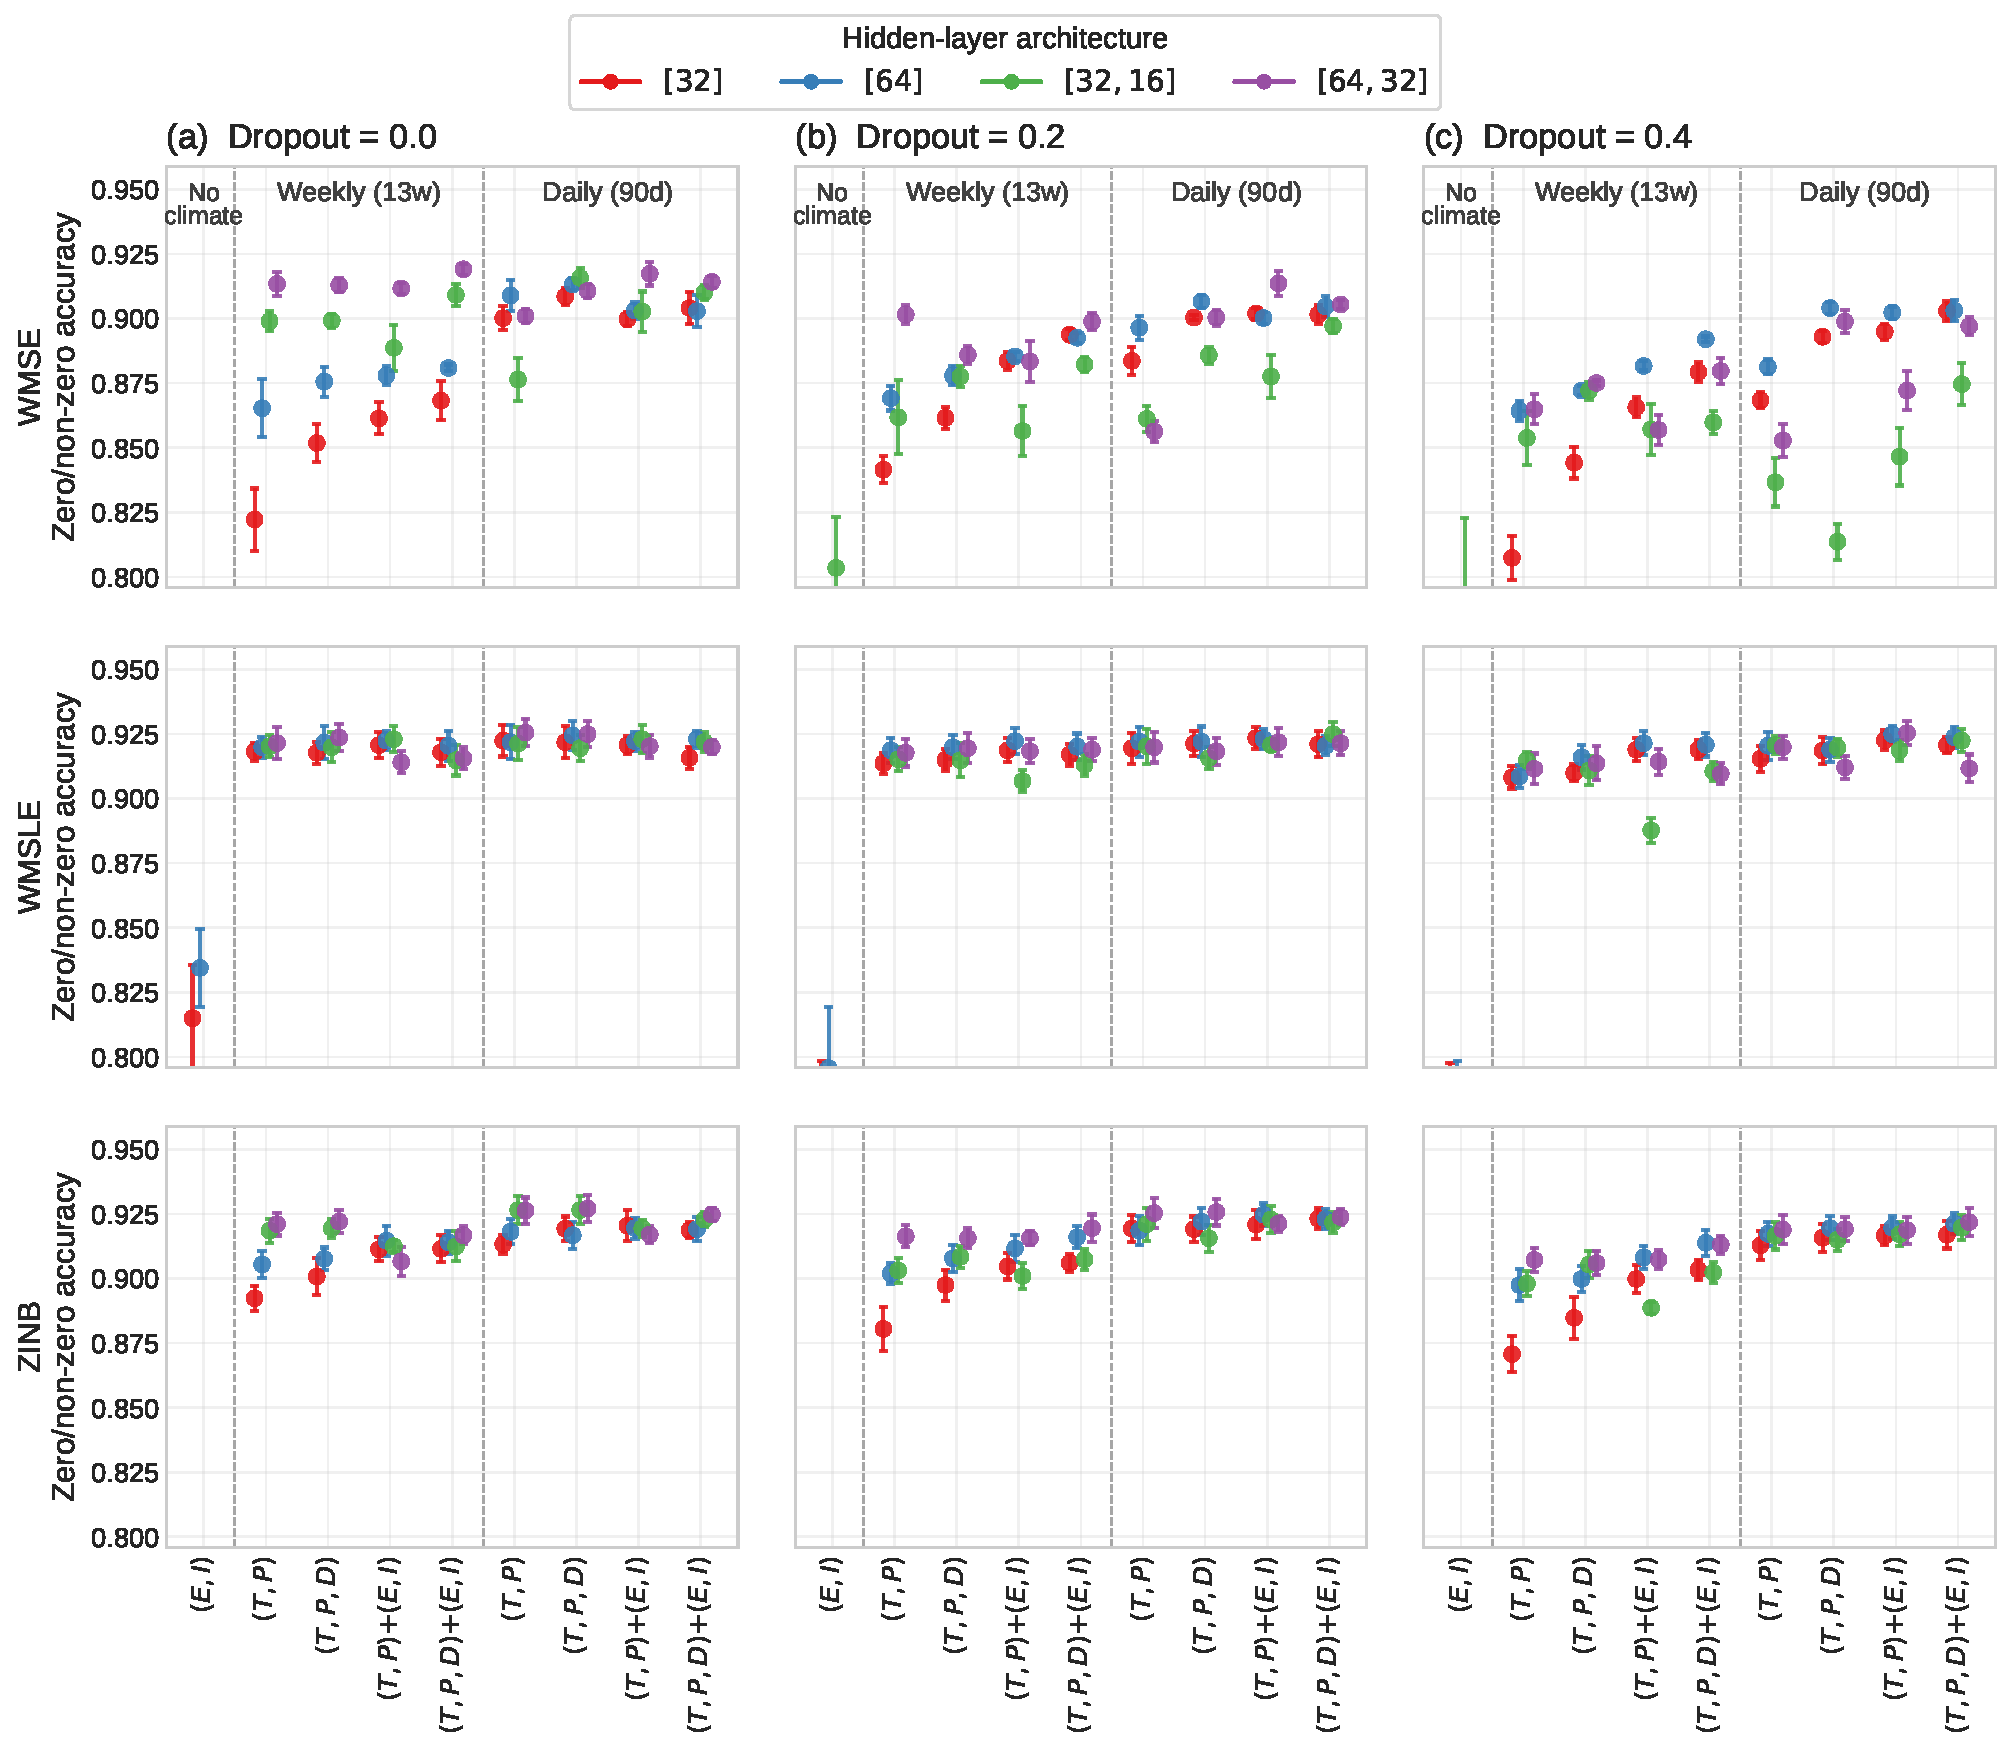
\includegraphics[width=0.8\linewidth]{img/nn_results_by_dropout_3loss_acc.pdf}
    \caption{Effect of dropout, network depth, and input variable combinations on test accuracy across three loss functions. WMSLE provided the highest overall classification accuracy, particularly when egg-laying rate features ($p1zn$, $p2zn$) were included.}
    \label{fig:loss_dropout_acc}
\end{figure}

\begin{table}
\centering
\caption{Best-performing configuration per loss function. Each entry reports the mean $\pm$ standard deviation across 20 seeds for $R^2$, classification accuracy, and RMSE, followed by architecture (dropout / layers / hidden units) and input variables.}
\label{tab:best_per_loss}
\begin{tabular}{l r r r l l}
\toprule
LossFn & $R^2$ & Acc & RMSE & DO/Lay/HU & Variables \\
\midrule
WMSE   & $0.643 \pm 0.005$ & $0.870 \pm 0.005$ & $22.8 \pm 1.5$ & 0.0/2/64 & {\small $AT_{13w}$\,\text{+}\,$TP_{13w}$\,\text{+}\,$ER_{2w}$} \\
WMSLE  & $0.629 \pm 0.005$ & $0.919 \pm 0.002$ & $22.6 \pm 1.2$ & 0.2/2/64 & {\small $AT_{90d}$\text{+}$TP_{90d}$\text{+}$DP_{90d}$\text{+}$ER_{2w}$} \\
ZINB   & $0.621 \pm 0.014$ & $0.918 \pm 0.002$ & $23.2 \pm 1.3$ & 0.4/3/64 & {\small $AT_{90d}$\text{+}$TP_{90d}$\text{+}$ER_{2w}$} \\
\bottomrule
\end{tabular}
\end{table}


\printbibliography

\end{document}